\subsection{
  Replies to comments received from Okumura-san - Aug 14, 2013 }

\begin{enumerate}

  % ........................................................................................................
  \vspace{5 mm}
\item
  {\em
    P10 Line 435:\\
    It is written that the uncertainty of $\theta_{13}$ is implemented in the fit by systematic parameter,
    and the uncertainty of $\delta_{CP}$ is included by throwing it randomly in the calculation of $\Delta \chi^2$ critical surface.
    I think that these different implementations may cause the cancellation of these systematic effect each other.
    As you know, both $\theta_{13}$ and $\delta_{CP}$ parameters can increase/decrease $\nu_\mu \rightarrow \nu_e$ oscillation.
    In the fitting procedure of toy-MC for critical $\chi^2$ value, assume that a toy MC is generated with
    a $\delta_{CP}$ value to enlarge $\nu_\mu \rightarrow \nu_e$ oscillation, then $\theta_{13}$ parameter should be moved so as to increase
    $\nu_\mu \rightarrow \nu_e$ oscillation to fit this toy MC distribution. And vice versa. As a result, some correlation is
    made between $\theta_{13}$ and $\delta_{CP}$, and systematic effect of $\delta_{CP}$ becomes under-estimated than expected I guess.
    Could you check for example, the correlation between generated $\delta_{CP}$ and fitted $\theta_{23}$ value?
  }\\
  \\
  No correlation has been found. See, for example,
  the correlation between generated $\delta_{CP}$ and fitted $\sin^2\theta_{23}$ residual
  in Fig.\ \ref{fig:dcp_sintheta23_correlation},
  and the correlation between generated $\delta_{CP}$ and fitted $|\Delta m^2_{32}|$ residual
  in Fig.\ \ref{fig:dcp_dm32sq_correlation} of this document.

  In v3 of the note, we will fit for $\delta_{CP}$ (see reply to Scott's comment 6).

  \begin{figure*}[htb]
    \begin{minipage}[t]{0.48\linewidth}
      \center
      \includegraphics[width=20pc]{{./images/dcp_sintheta23_correlation_0.37}.eps}
      \caption {
        Correlation between the input $\delta_{CP}$ value and the fitted
        $\sin^2\theta_{23}$ residual,
        computed from 5.1k toy MC experiments at $6.3933\times10^{20}$ POT,
        generated at
        at $\sin^2\theta_{23} = 0.37$ and $|\Delta m^2_{32}| = 2.4\times10^{−3}$ eV$^2$/c$^4$, including
        statistical fluctuations and with randomized systematic parameters.
      }
      \label{fig:dcp_sintheta23_correlation}
    \end{minipage}
    \hspace{0.06\linewidth}
    \begin{minipage}[t]{0.48\linewidth}
      \center
      \includegraphics[width=20pc]{{./images/dcp_dm32sq_correlation_0.37}.eps}
      \caption {
        Correlation between the input $\delta_{CP}$ value and the fitted
        $|\Delta m^2_{32}|$ residual,
        computed from 5.1k toy MC experiments at $6.3933\times10^{20}$ POT,
        generated at
        at $\sin^2\theta_{23} = 0.37$ and $|\Delta m^2_{32}| = 2.4\times10^{−3}$ eV$^2$/c$^4$, including
        statistical fluctuations and with randomized systematic parameters.
      }
      \label{fig:dcp_dm32sq_correlation}
    \end{minipage}
  \end{figure*}
  

  % ........................................................................................................

  \vspace{5 mm}
\item
  {\em
    P18 Table 3:\\
    It is written that you take the uncertainty of $\sin^2(\theta_{13})$ from PDG.
    But our T2K $\nu_e$ result using same RUN1-4 dataset gives larger $\theta_{13}$ best-fit value,
    and it is out of the uncertainty range you set. Since this analysis use same dataset as $\nu_e$,
    I'm not sure that this assumption is okay or not.
    I'm not sure that our best fit value of $\theta_{13}$ is due to effect of $\delta_{CP}$ or $\theta_{23}$,
    but we obtained this large $\theta_{13}$ with the assumption of $\delta_{CP}$=0 and $\sin^2(\theta_{23})=0.5$.
    In your $\nu_\mu$ analysis, this condition is similar I think; you apply fit with $\delta_{CP}$=0.
    Since we measured $\nu_\mu \rightarrow \nu_e$ oscillation more than expected by PDG value in the same dataset,
    isn't it better to take $\theta_{13}$ uncertainty in a consistent way with our $\nu_e$ result ?
    According to Figure 14, the uncertainty of $\theta_{13}$ is seen around oscillation peak,
    I guess it affect to $\sin^2(\theta_{23})$ uncertainty and it may be under-estimated.
  }\\
  \\
  In v3 of the note, we plan to fit for $\delta_{CP}$ (see reply to Scott's comment 6).
  Therefore we feel that using the reactor data is the natural choice,
  as this allows us to use a single number for the constraint term of $\sin^2\theta_{13}$ -
  if we used the T2K result we would need a multi-dimensional likelihood function
  to evaluate the correct $\sin^2\theta_{13}$ error for the penalty at the current value of
  $\sin^2\theta_{23}$ and $\delta_{CP}$.
  Using reactor data also prevents any correlations between $\nu_e$ and $\nu_\mu$ T2K
  data effecting the result.
  
  % ........................................................................................................

  \vspace{5 mm}
\item
  {\em
    P26 Table 7:\\
    You showed $\delta N_{sk}$/$N_{sk}$ for both BANFF prefit and postfit.
    I understand that errors related to BANFF parameters are reduced for postfit,
    but I don't understand that other errors are reduced largely. for example, that of
    $f_{\pi-less\Delta; t, r}$ changed from 6.3 to 4.9, $f_{NC1\pi^\pm; t}$ changed from 1.1 to 0.78.  Could you explain why ?
  }\\
  \\
  This is due to the fact that the BANFF fit changes the nominal spectrum, in addition to the size of the errors.
  Taking the example of $f_{NC1\pi^\pm; t}$,
  in the prefit case, the contribution to the total $N_{SK}$ from $NC1\pi^\pm$ modes is 3.21\%,%3.211806\%,
  and 40\% of this (the 1$\sigma$ $f_{NC1\pi^\pm; t}$ error) is 1.28\%.
  In the postfit case, the contribution to the total $N_{SK}$ from $NC1\pi^\pm$ modes is 2.60\%,%2.595826\%,
  and 40\% of this is 0.78\%.

  It is difficult to present a simple argument to confirm that $f_{\pi-less\Delta; t, r}$ is behaving correctly
  since it has both an $E_{reco}$ and $E_{true}$ dependence.
  % Contrib from modes PRE:                                      1pi :       41.235711 events ( 32.265295 \%)
  % Contrib from modes POST:                                     1pi :       36.017760 events ( 30.581505 \%)

  It should be noted that the prefit column of Tab.\ 10 of TN141
  is a direct copy of the postfit column, for all but the BANFF parameters.

  % ........................................................................................................

  \vspace{5 mm}
\item
  {\em
    P26 Table 7:\\
    You estimate $N_{sk}$ error due to $\delta_{CP}$ in this table. Could you explain how you estimate?
    You throw many toy MC with random $\delta_{CP}$, make $N_{sk}$ distribution, and take 1 sigma width of it? 
    Did you use this value in somewhere of your analysis program?
  }\\
  \\
  For the table in v1, the value is the maximum deviation of $\pm\pi/2$ tweaks.
  We agree that this is not the best thing to do for this parameter,
  therefore in v2 it is the 1 $\sigma$ width of 10000 uniform throws between $-\pi$ and $+\pi$.
  
  Note that for other parameters, the values were taken from the maximum deviation of $\pm1\sigma$ tweaks.
  This has been updated in v2 for parameters using splines, and oscillation parameters
  (parameters which are not pure normalisations)
  to use the same throw-based method.
  This was the same method that was used in Tab.\ 10 of TN141.
  
  % ........................................................................................................

  \vspace{5 mm}
\item
  {\em
    P39 Figure 45 \& 46:\\
    Can you compare these to those of previous analysis (TN-148)?
    I noticed that $f_{E; r}^{SK}$ pull deviates from zero this time while it was close to zero previously. Can you explain why?
  }\\
  \\
  A full comparison is not possible, since the SuperK detector efficiency \& FSI+SI parameters were separate in
  TN141.
  A comparison of SK energy scale, BANFF, and uncorrelated cross section parameters is shown in
  Fig.\ \ref{fig:compare_pulls} of this document, for 3 fits to the Run 1-3 data:
  \begin{itemize}
  \item TN141 method, 2012 SK data analysis;
  \item TN155 method, 2012 SK data analysis;
  \item TN155 method, 2013 SK data analysis.
  \end{itemize}
  The difference between 2012 and 2013 SK data analysis is described in
  TN148; for 1-ring $\mu$-like events, the effect is a spectrum change,
  two additional event accepted and one additional event rejected in 2013.
  All results assume normal mass hierarchy.
  
  The figure shows that differences in the pull distributions is due to a combination of
  two sources: 
  the differences betweens the TN141 \& TN155 fitters;
  and the difference in the SK energy spectrum for Run 1-3.

  We also refer you to the answer to Scott's question 9 - the error from the fit produced for $f_{E; r}^{SK}$
  is not as accurate as for the other parameters.
  
  \begin{figure*}[htb]
    \center
    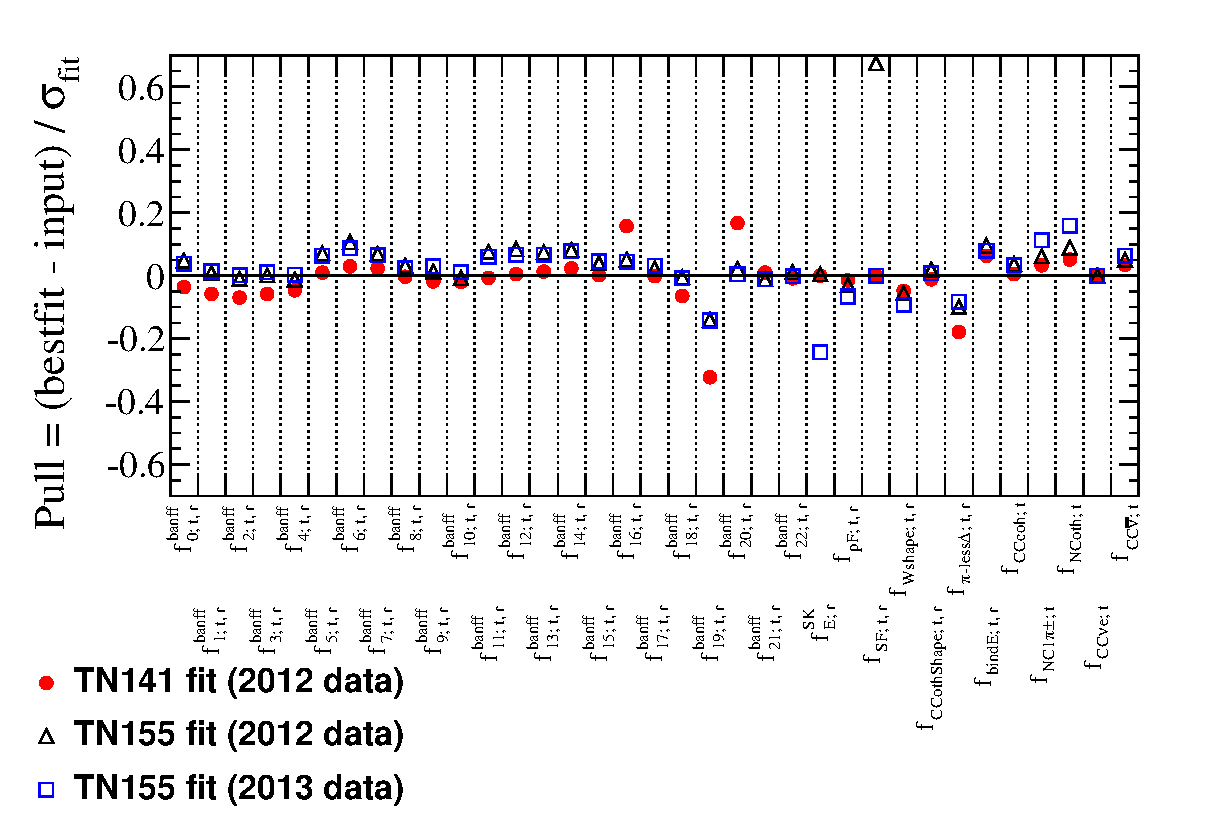
\includegraphics[width=30pc]{./images/pulls_comparison}
    \caption {
      Systematic parameter pulls for the fits to the Run 1+2+3 dataset.
      Results using the method of TN141 (2012 SK data analysis) and TN155 (2012 \& 2013 SK data analyses) are shown.
      The normal mass hierarchy is assumed.
    }
    \label{fig:compare_pulls}
  \end{figure*}


  % ........................................................................................................

  \vspace{5 mm}
\item
  {\em
    P57 Figure 69:\\
    You compared contours for const-$\Delta\chi^2$ and FC method. In page 10 Line 435, you described
    "the effect of $\delta_{CP}$ is handled by throwing ...."  Then I understand that the uncertainty
    due to $\delta_{CP}$ is included only in contour by FC method.
    Though it is not easy to compare in Fig 69 due to that FC analysis is not completed, it seems that
    there is not large difference between two contours due to $\delta_{CP}$. Is the effect of $\delta_{CP}$
    negligibly small ? Is it possible to quantify the effect of $\delta_{CP}$ ?
  }\\
  \\
  Please see the reply to Scott's comment 6.
  

  % ........................................................................................................



\end{enumerate}

